\chapter[Avaliação de Capacidade]{Avaliação de Capacidade}
% ----------------------------------------------------------
Dadas as definições e formalizações propostas no anteriormente, faz-se necessária
a especificação de uma lógica de manipulação das entidades e operações descritas.

Passamos agora a descrever uma proposta de processo de avaliação de capacidade
que visa a buscar as Configurações de menor preço capazes de executar uma determinada 
Carga de Trabalho. Esse processo foi implementado como parte de um sistema 
computacional ao qual demos o nome de \emph{Cloud Capacitor} e que descreveremos 
no capítulo seguinte.  

O processo prevê um conjunto de dados de entrada, ao menos uma execução da 
Aplicação sob Teste no ambiente de nuvem de infraestrutura almejado para 
hospedá-la, e, por fim, a análise do desempenho obtido pela Aplicação a partir 
de suas execuções. Com base nos dados de desempenho, o processo passa por diversos
pontos de decisão que podem levar a novas execuções da Aplicação em diferentes 
cenários. Ao final do processo, é fornecida como saída uma lista de Configurações, 
ordenadas por preço, capazes de executar a Aplicação sob Cargas de Trabalho específicas.

Este capítulo estuda em detalhes todas as fases do processo de avaliação de capacidade
proposto, explicando quais são os dados de entrada necessários, os componentes do 
processo e as operações pelas quais são responsáveis e quais as decisões pelas quais
o processo tem que passar até determinar quais são as Configurações de menor custo
capazes de executar a Aplicação.

\section{Dados de Entrada}

O principal parâmetro esperado pelo processo de avaliação de capacidade é o Valor
de Referência de Desempenho, ao qual também nos referimos como SLA 
(\emph{Service Level Agreement}). Esse valor será usadp para determinar 
se a Aplicação atingiu os requisitos mínimos de desempenho exigidos, conforme
veremos na descrição do funcionamento do processo, mais adiante.

Além do SLA, o processo precisa também conhecer quais são as Cargas de Trabalho
que deverão ser submetidas à Aplicação sob Teste durante seu funcionamento. Porém,
nem todas as Cargas de Trabalho serão submetidas de fato. Isso vai depender do 
conjunto de decisões tomadas pelo processo com base na comparação do desempenho 
da Aplicação com o SLA. Ainda assim, graças à sua característica de inferência de
desempenho, o processo mostra resultados para todas as Cargas de Trabalhado 
informadas como parâmetro de entrada.

Para que a Aplicação seja executada, é preciso que o processo conheça quais são
as Configurações disponibilizadas no Provedor de nuvem para esse fim. Para isso,
o processo deve ser alimentado com uma lista de Tipos de Máquinas Virtuais que
serão utilizadas na execução da Aplicação, bem como a quantidade máxima de 
instâncias usadas para compor cada Configuração. Através desses dados o processo
passa a conhecer então o Espaço de Implantação disponível para os testes de 
desempenho, composto por uma lista de Configurações geradas a partir da lista de
Tipos de Máquinas Virtuais disponíveis e do número máximo de instâncias.

\section{Funcionamento do Processo}

O processo de avaliação de capacidade proposto é um processo extensível, ao qual
devem ser ligados componentes para os quais são delegadas funções de cunho mais
específico, como a comunicação com o Provedor de nuvem e a Aplicação sob Teste
para fins de orquestração do teste de desempenho, e também funções para as quais
é desejado um certo grau de flexibilidade a fim de tornar o processo mais adaptável,
como a escolha das Cargas de Trabalho e Configurações que serão usadas na execução
da Aplicação.

\begin{figure}[htb]
  \caption{\label{fig_processo_alto_nivel}Visão geral do Processo de Avaliação de Capacidade}
  \begin{center}
    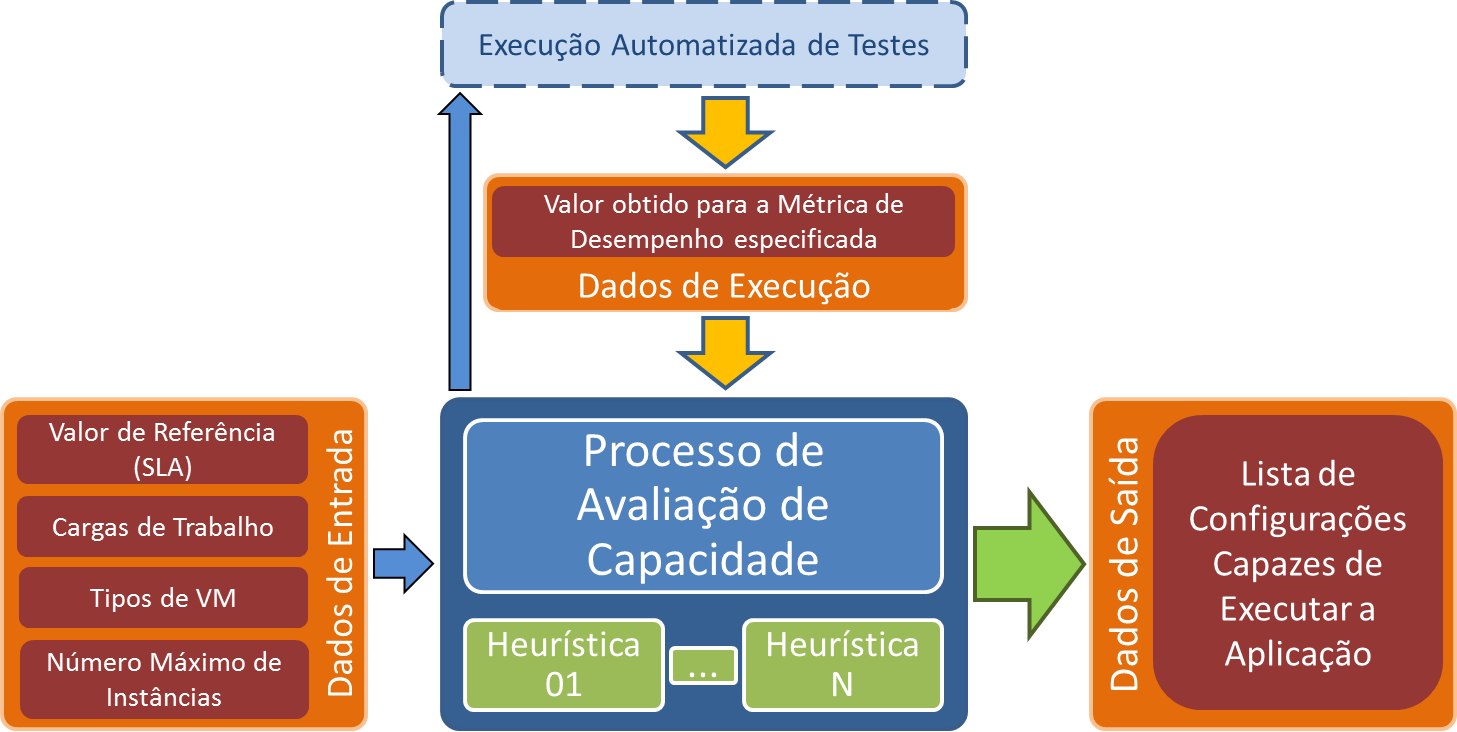
\includegraphics[scale=0.5]{img/processoAltoNivel}
  \end{center}
\end{figure}

Toda a rotina de execução da Aplicação, desde sua implantação, passando pela 
criação e configuração das máquinas virtuais no ambiente do Provedor de nuvem, 
bem como pelo controle de inicialização e finalização dessas instâncias, serviços
subjacentes como bancos de dados e filas, e a própria parametrização da execução
e parada da Aplicação em si, não fazem parte do escopo do processo. Todas essas
operações são delegadas a um componente que chamamos de Executor. 

O processo considera que existe um Executor que conhece os detalhes inerentes à 
Aplicação sob Teste e é capaz de ordenar a sua execução e coletar como resposta
os dados de desempenho esperados pelo processo.

Analogamente, as operações de seleção de uma Configuração sobre a qual a Aplicação
so Teste será executada e seleção da Carga de Trabalho a que ela será submetida 
durante sua execução são delegadas a um componente que chamamos de Estratégia de
Avaliação ou, simplesmente, Estratégia. Neste caso, porém, o objetivo é permitir
que diferentes estratégias apliquem métodos próprios para a escolha da melhor 
Configuração e/ou Carga de Trabalho mais adequada aos objetivos da avaliação de
capacidade em curso e também ao perfil da Aplicação.

Dessa forma, o processo permite que a mesma Aplicação seja facilmente avaliada 
por meio de diferentes abordagens e sem modificação da lógica geral original de 
avaliação. Para exemplificar, uma Estratégia pode selecionar Configurações 
maiores ou menores priorizando a escalabilidade vertical em detrimento da mudança
do número de instâncias que compõem a Configuração anterior. Outra Estratégia 
poderia agir da mesma maneira, mas levando em consideração o consumo de CPU e/ou
memória apresentado pela Aplicação com base nos dados de desempenho coletados a
partir da sua execução anterior.

\begin{figure}[htb]
  \caption{\label{fig_processo_aval_capacidade}Diagrama de Funcionamento do Processo de Avaliação de Capacidade}
  \begin{center}
    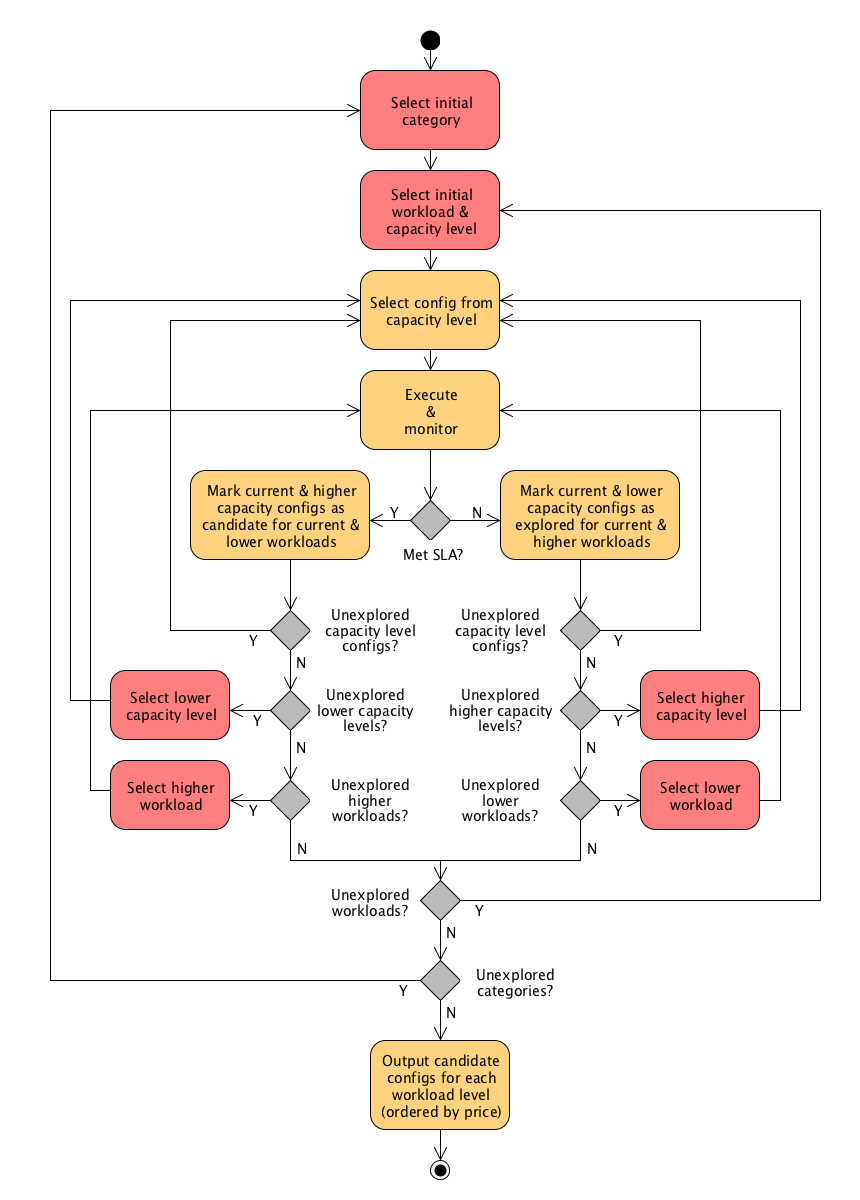
\includegraphics[scale=0.4]{img/diagrama-avaliacao-capacidade-v14}
  \end{center}
\end{figure}

Para efeito de entendimento do funcionamento do processo de avaliação de capacidade
ora proposto, podemos abstrair o comportamento dos componentes Executor e 
Estratégia de Avaliação. Esta é, aliás, outra vantagem da abordagem adotada de 
delegação de funções específicas a componentes: além da flexibilidade e 
adaptabilidade, a abstração as operações torna mais fáceis o entendimento, a 
descrição e a implementação concreta do processo.   

Na Figura~\ref{fig_processo_aval_capacidade}, os blocos em vermelho representam
as operações que o processo espera que sejam executadas por uma Estratégia de 
Avaliação. A delegação de funções para o Executor não está destacada e se dá no
passo ``\emph{Execute \& Monitor}''.

\subsection{Operações Iniciais}
Para que uma Heurística de Avaliação de Capacidade seja compatível no âmbito deste trabalho, 
deve apresentar um conjunto mínimo de operações esperadas para que a lógica da
avaliação se complete e o resultado final obtido possa ser considerado válido e
comparável com os resultados obtidos por outras Heurísticas.

Além disso, as operações constituem a interface pela qual o controlador das 
sessões de avaliação pode configurar as Heurísticas e informar-lhe os dados 
necessários ao controle da sua execução.
 
Apresentamos esse conjunto mínimo de operações nas subseções a seguir, que 
representam o arcabouço necessário para a construção de uma Heurística de 
Avaliação de Capacidade.

\subsubsection{Selecionar Carga de Trabalho Inicial}
Este trabalho tem como premissa a necessidade de se identificar quais as 
Configurações mais baratas em um Provedor capazes de executar diversos níveis de
Cargas de Trabalho, tendo como objetivo a otimização de custos para a execução de
uma Aplicação so Teste.

Assim, pressupomos que exista uma faixa de valores para os níveis de Cargas de 
Trabalho a que a Aplicação é costumeiramente submetida e que seja de conhecimento
prévio dos responsáveis pela Aplicação. 

De posse dessa faixa de valores de Cargas de Trabalho, uma Heurística deve ser 
capaz de escolher, de acordo com sua estratégia de trabalho, um valor inicial de
Carga de Trabalho a ser imposta sobre a Aplicação. A Carga de Trabalho escolhida
deve ser retornada para o controlador da sessão, de forma que este possa coordenar
a Execução dos testes.
 
\subsubsection{Selecionar Configuração Inicial}
Analogamente, a fim de que as atividades da sessão de avaliação possam ter início,
é necessário que a Heurística de Avaliação de Capacidade usada selecione uma
Configuração inicial.

A escolha da Configuração inicial é feita a partir das Configurações disponíveis
no Espaço de Implantação previamente configurado pelo responsável pela avaliação.
A Heurística deverá avaliar o conjunto de configurações disponíveis quanto ao seu
preço, número de instâncias em cada, etc, de forma a escolher uma Configuração 
que considere mais adequada à sua estratégia para o início da sessão de avaliação.

\subsection{Operações de Controle}
Tendo em mãos uma Carga de Trabalho e uma Configuração iniciais, o controlador
da sessão de avaliação de capacidade pode ordenar uma Execução de testes, onde
serão coletados dados de desempenho relevantes para a Aplicação sob Teste.

Após a primeira Execução, um Resultado contendo os dados de desempenho colhidos 
é avaliado pelo controlador e, conforme sua decisão, novas Execuções podem se 
fazer necessárias. Neste caso, a Heurística deve ser novamente invocada, desta 
vez a selecionar uma nova Carga de Trabalho ou uma nova Configuração a partir do
Espaço de Implantação. Essa interação deve se repetir até que o controlador 
conclua os testes e dê por encerrada a sessão de avaliação.

Abaixo descrevemos as operações que a Heurística deve prover para que permita ao
controlador a correta operação dos testes e da sessão.

\subsection{Selecionar Nova Configuração}
Depois da cada execução de testes, o controlador estará de posse de um Resultado,
contendo os dados de desempenho da Aplicação executada sob a Carga de Trabalho e
a Configuração selecionadaa. A depender dos dados desse Resultado, o controlador
pode decidir executar novos testes em outra Configuração.

Para isso, a Heurística deve ser usada para selecionar a próxima Configuração a 
ser testada com a Aplicação. Com base no Resultado obtido pela Execução anterior,
a Heurística usará sua lógica de navegação para determinar a distância a ser 
caminhada no Espaço de Implantação em busca da nova Configuração.

A ordem de caminhamento é dada conforme a necessidade identificada pelo 
controlador, que vai definir se precisa de uma Configuração mais ou menos potente.
Porém, a Heurística é quem define, através de sua estratégia, qual será a próxima
Configuração usada.

Assim, a Heurística deve prover ao controlador duas operações para escolha da 
próxima Configuração: uma para Elevar o Nível de Configuração, ou seja, escolher
uma Configuração de capacidade superior, e outra para Reduzir o Nível de 
Configuração, isto é, escolher uma Configuração de capacidade inferior. Em ambos
os casos, a Heurística deverá usar como dado de entrada o Resultado da última 
Execução.

As Heurísticas são livres para usar os dados do Resultado como melhor lhe 
aprouverem, desde que a saída seja uma Configuração que ainda não tenha sido 
usada nos testes anteriores. 

\subsection{Selecionar Nova Carga de Trabalho}
De maneira similar à escolha de uma nova Configuração, o controlador pode usar
a Heurística para selecionar uma nova Carga de Trabalho, de acordo com o 
resultado com a última Execução.

As Heurísticas devem, então, prover operações que permitam a navegação pela
faixa de valores de Cargas de Trabalho estudada para a Aplicação sob Teste. 
Portanto, uma Heurística compatível deve fornecer duas operações de controle do
nível de Carga de Trabalho: uma operação para que seja reduzido e outra operação 
para que seja elevado o nível de Carga de Trabalho.

Aqui também as Heurísticas são livres para criarem suas próprias lógicas de 
avaliação dos dados do Resultado e, a partir daí, definirem qual o tamanho do
passo no caminhamento sobre a faixa de Cargas de Trabalho.
 
% ----------------------------------------------------------
